%\documentclass[aspectratio=169]
\documentclass[aspectratio=169,xcolor=dvipsnames]{beamer}
%\usetheme{Copenhagen}
\usetheme{Madrid}
\setbeamertemplate{navigation symbols}{}
%\setbeamertemplate{footline}{}
\usecolortheme[named=Green]{structure}

\usepackage[utf8]{inputenc}

\usepackage{graphicx}         
\graphicspath{ {./Pictures/} }
\usepackage{amsmath}
\usepackage{amsfonts}
\usepackage{amssymb}
\usepackage{amsthm}
\usepackage{mathtools}
\usepackage{commath}
\usepackage{multimedia}
\usepackage{subcaption}
\usepackage{media9}
\addmediapath{Animations/}
\newcommand{\Sta}{y}
\newcommand{\Adj}{p}
\newcommand{\Con}{u}
\begin{document}
 \author[Jonna Roden (UoE)]{Jonna Roden (UoE)}
 \title[Supervision: Ben Goddard, John Pearson]{With Dr Ben Goddard (UoE), Dr John Pearson (UoE)}
 \date{May 11, 2020}
 
\begin{frame}
	\frametitle{PDE-Constrained Optimization for Multiscale Particle Dynamics}
	 \begin{align*}
	 &\min_{\rho,\mathbf{w}} \ \  \frac{1}{2}||\rho - \widehat \rho||_{L^2}^2 + \frac{\beta}{2}||\mathbf{w}||_{L^2}^2\\
	 &\text{subject to:}\\
	 &\partial_t \rho = \Delta \rho - \nabla \cdot (\rho\mathbf{w} ) + \nabla \cdot \int_\Omega \rho(\mathbf{x}) \rho(\mathbf{x'})\nabla V_2(|\mathbf{x}-\mathbf{x'}|)d\mathbf{x} \quad + \text{ BC } + \text{IC}
	 \end{align*}
	 \vspace{-0.5cm}
	 \begin{figure}
	 	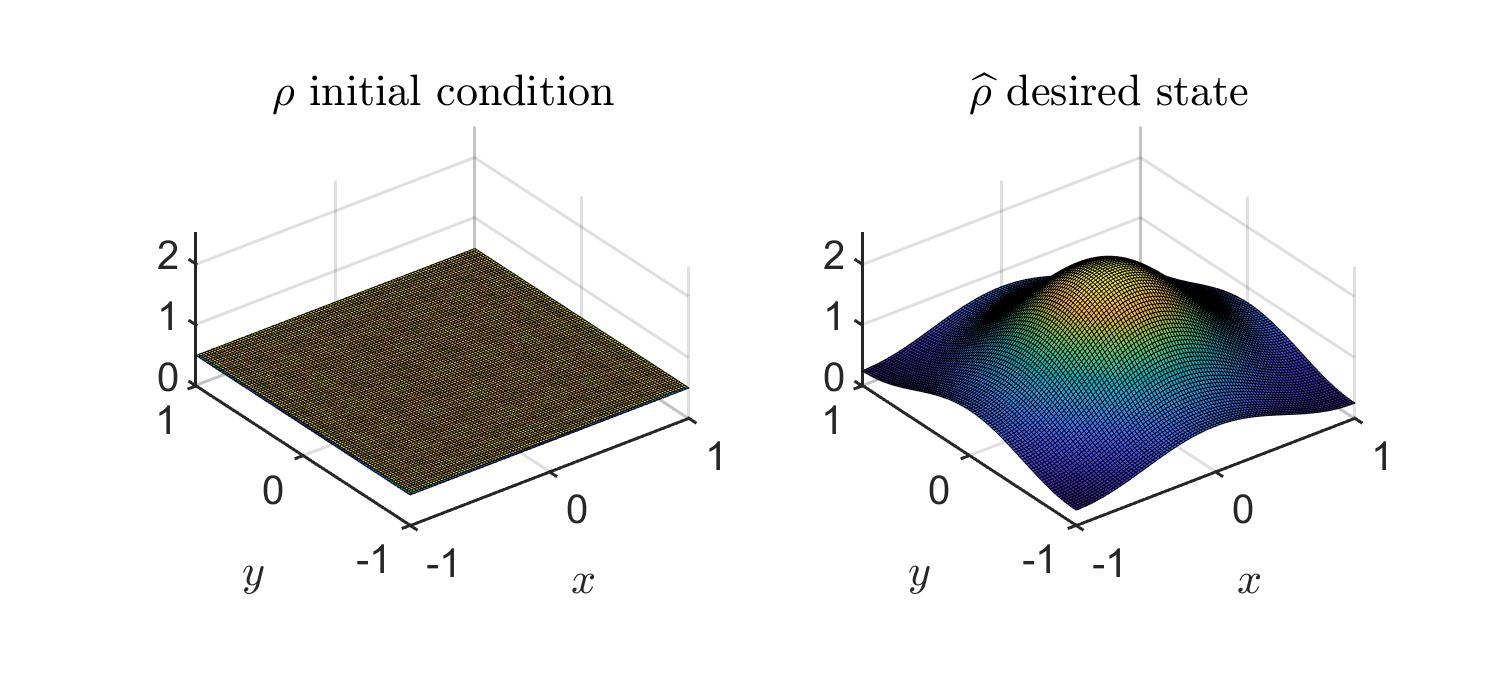
\includegraphics[width=11cm]{Example2.jpg}
	 	%\caption{ Nanofiltration Device}
	 \end{figure}
\end{frame}


\end{document}